% Generated by scripts/supp_tex.py from scripts/supp/d_full_results.py.
% Do not edit: edit the module, which also builds the PDF version.

\section{Complete results}
\label{supp:d_full_results}

This section prints in full what the main paper samples: every class at every quality index and at three budgets, the frontier drawn class by class, and the distribution behind each mean, over sequences and over tiles. It also carries three measurements the main paper has no room for: a perceptual metric beside the decibel, the composition with weight quantisation, and the raw numbers behind the curves. It ends with the cases where the method does badly.

\subsection{Every class at every rate}

\begin{table}[t]
\centering
\resizebox{\columnwidth}{!}{%
\begin{tabular}{lrrrrr}
\toprule
Class & q0 & q16 & q32 & q48 & q63 \\
\midrule
MCL-JCV & 37.1 & 34.4 & 31.2 & 30.2 & 29.2 \\
UVG & 36.0 & 33.8 & 31.2 & 28.3 & 26.7 \\
HEVC B & 34.9 & 31.3 & 25.1 & 21.9 & 19.4 \\
HEVC E & 36.6 & 32.4 & 29.3 & 29.3 & 29.3 \\
HEVC C & 25.6 & 17.1 & 7.8 & 6.6 & 4.8 \\
HEVC D & 18.3 & 10.9 & 2.5 & 2.5 & 2.5 \\
All \NumSeq, pooled & 34.4 & 30.8 & 26.6 & 25.2 & 24.1 \\
Quality given up (dB) & 0.100 & 0.100 & 0.099 & 0.099 & 0.100 \\
\bottomrule
\end{tabular}}
\caption{Compute saved against the released decoder, by class and by quality index, at the 0.1 dB budget; the main paper prints the q0, q32 and q63 columns of the first six rows. Read it in two directions. Along a row the saving falls with rate, because the residual a shallow exit fails to reconstruct grows relative to the quality being protected. Down a column it falls with resolution, from \BigResLow\% on MCL-JCV to \SmallResLow\% on HEVC D at q0, because a 256 px tile is 40 tiles on a 1080p frame and two at 416x240. The last row is the quality the pooled allocation gave up, which is the budget to within a thousandth of a decibel at every rate.}
\end{table}

{\small results/supp\_per\_class\_budgets.json, on runs/RECIPE512/ckpt\_PAPER.pth.tar, \NumSeq sequences at one frame each, per-frame convention. The pooled row reads 29.7\% at q0 where the main paper's \MainLowRate\% comes from results/signalled\_RECIPE512\_ctc53.json; the two bisect the same budget with different code and settle on $\lambda$ = 5.126$\times$10$^{-5}$ and 5.150$\times$10$^{-5}$.}

\begin{figure}[t]
\centering

\includegraphics[width=\columnwidth]{figures/res_grid.png}
\caption{The same measurement as a grid, with the looser budget under it. \textbf{a}, compute saved at the 0.1 dB budget. \textbf{b}, the same at 0.3 dB, where every class at the three lowest rates has reached the architectural ceiling of \CeilingModelled\% and only q48 and q63 are still making a choice. \textbf{c}, the quality actually given up at the 0.1 dB budget, which the set meets and no class does: at q0 the allocation spends 0.116 dB on MCL-JCV and 0.028 dB on HEVC D. The small classes are cheap in quality for the same reason they are poor in saving, that with two or eight tiles there is no fine-grained way to spend a budget. The 0.5 dB grid is not drawn because every one of its thirty cells is at the ceiling.}
\end{figure}

{\small Drawn by scripts/supp\_results\_figs.py from results/supp\_per\_class\_budgets.json, on runs/RECIPE512/ckpt\_PAPER.pth.tar.}

The resolution effect is a property of the tiling and not of the content, which is the argument against reading a single mean over a test set that mixes resolutions: MCL-JCV is 30 of the \NumSeq sequences and all of them 1080p, so it carries most of the pooled row.

\subsection{Adaptivity against its controls}

The main paper prints this comparison transposed and compressed to five columns. The full form is below, one block per quality index, because the uniform rows are the ones a reader is most likely to want to read off directly: they say what a decoder that made no per-tile choice at all would deliver at the same budget.

\begin{table}[t]
\centering
\resizebox{\columnwidth}{!}{\begin{tabular}{llrr}
\toprule
$q$ & Allocation & $\Delta$PSNR (dB) & MACs saved (\%) \\
\midrule
0 & uniform, exit 2$^{\dagger}$ & 0.139 & 39.1 \\
 & uniform, exit 3 & 0.061 & 24.2 \\
 & uniform, exit 4 & 0.041 & 13.0 \\
 & uniform, exit 5 & 0.026 & -1.0 \\
 & random (matched mix) & 0.114 & 34.5 \\
 & rate-ranked (free) & 0.104 & 34.5 \\
 & \textbf{oracle} & \textbf{0.100} & \textbf{34.5} \\
\midrule
16 & uniform, exit 2$^{\dagger}$ & 0.172 & 39.1 \\
 & uniform, exit 3 & 0.080 & 24.2 \\
 & uniform, exit 4 & 0.055 & 13.0 \\
 & uniform, exit 5 & 0.034 & -1.0 \\
 & random (matched mix) & 0.123 & 30.8 \\
 & rate-ranked (free) & 0.104 & 30.8 \\
 & \textbf{oracle} & \textbf{0.100} & \textbf{30.8} \\
\midrule
32 & uniform, exit 2$^{\dagger}$ & 0.218 & 39.1 \\
 & uniform, exit 3$^{\dagger}$ & 0.105 & 24.2 \\
 & uniform, exit 4 & 0.067 & 13.0 \\
 & uniform, exit 5 & 0.042 & -1.0 \\
 & random (matched mix) & 0.134 & 26.7 \\
 & rate-ranked (free) & 0.105 & 26.7 \\
 & \textbf{oracle} & \textbf{0.100} & \textbf{26.7} \\
\midrule
48 & uniform, exit 2$^{\dagger}$ & 0.253 & 39.1 \\
 & uniform, exit 3$^{\dagger}$ & 0.122 & 24.2 \\
 & uniform, exit 4 & 0.074 & 13.0 \\
 & uniform, exit 5 & 0.048 & -1.0 \\
 & random (matched mix) & 0.142 & 25.3 \\
 & rate-ranked (free) & 0.107 & 25.3 \\
 & \textbf{oracle} & \textbf{0.100} & \textbf{25.3} \\
\midrule
63 & uniform, exit 2$^{\dagger}$ & 0.288 & 39.1 \\
 & uniform, exit 3$^{\dagger}$ & 0.138 & 24.2 \\
 & uniform, exit 4 & 0.081 & 13.0 \\
 & uniform, exit 5 & 0.054 & -1.0 \\
 & random (matched mix) & 0.147 & 24.1 \\
 & rate-ranked (free) & 0.111 & 24.1 \\
 & \textbf{oracle} & \textbf{0.100} & \textbf{24.1} \\
\bottomrule
\end{tabular}
}
\caption{\textbf{Adaptivity against two controls} at the 0.1 dB budget, in full. Uniform rows are every tile at one depth. The dagger marks a uniform depth whose distortion exceeds the budget, so it is not an admissible allocation at all: at q48 and q63 the only uniform depth inside the budget is the deepest one, which costs \DeepestUniformCost\% rather than saving anything. \emph{Random} draws each frame's map from the oracle's own exit histogram and shuffles it across tiles, so the mix of depths and the average cost are unchanged and only the content dependence is discarded. \emph{Rate-ranked} keeps that histogram and orders it by the bits the entropy model spent per tile. Both shuffled rows are matched to the oracle on compute, so they are compared on the decibel column and not on the saving column.}
\end{table}

{\small results/static\_RECIPE512\_b01.json, on runs/RECIPE512/ckpt\_PAPER.pth.tar, seed recorded in the file, generated into paper/tables/static.tex by scripts/make\_paper\_tables.py.}

Two readings follow from the shuffled rows and they are easy to conflate. Quality falls sharply when the same histogram is assigned at random, so what the allocation buys is knowing \emph{which} tiles can afford to run shallower and not the fact that some fraction of them does. And ordering that same histogram by a free decoder-side signal recovers \RateRankRecovers\% of the oracle's advantage over chance at q63, which is the control section F turns into a complete routing rule.

\subsection{Where the tiles exit}

\begin{table}[t]
\centering
\resizebox{\columnwidth}{!}{%
\begin{tabular}{lrrrrrr}
\toprule
Rate & e2 & e3 & e4 & e5 & Blocks skipped & Saved \\
\midrule
q0 & 84.0 & 13.5 & 2.1 & 0.5 & 5.62 & 34.4 \\
q16 & 71.7 & 18.8 & 7.0 & 2.6 & 5.19 & 30.8 \\
q32 & 60.2 & 20.7 & 10.8 & 8.3 & 4.66 & 26.6 \\
q48 & 55.3 & 19.6 & 15.8 & 9.3 & 4.42 & 25.2 \\
q63 & 50.1 & 21.5 & 18.5 & 9.9 & 4.24 & 24.1 \\
\bottomrule
\end{tabular}}
\caption{The exit histogram at the 0.1 dB budget, as a percentage of the 1765 tiles in one pass over the test set, with the mean number of trunk blocks skipped and the saving that buys. At q0 two thirds of tiles take the shallowest selectable exit and the ladder above it is barely used. At q63 the mass is spread almost evenly over the four exits and the mean depth skipped has fallen from 5.04 blocks to 2.82. Exits e0 and e1 are omitted because the exit clamp cannot select them: the split depth is 2, so a map naming a shallower exit runs to e2 and wears e2's adapter.}
\end{table}

{\small Histograms summed over the six classes of results/supp\_per\_class\_budgets.json, on runs/RECIPE512/ckpt\_PAPER.pth.tar. Blocks skipped per exit from results/adapter\_cost.json, same checkpoint.}

\begin{figure}[t]
\centering
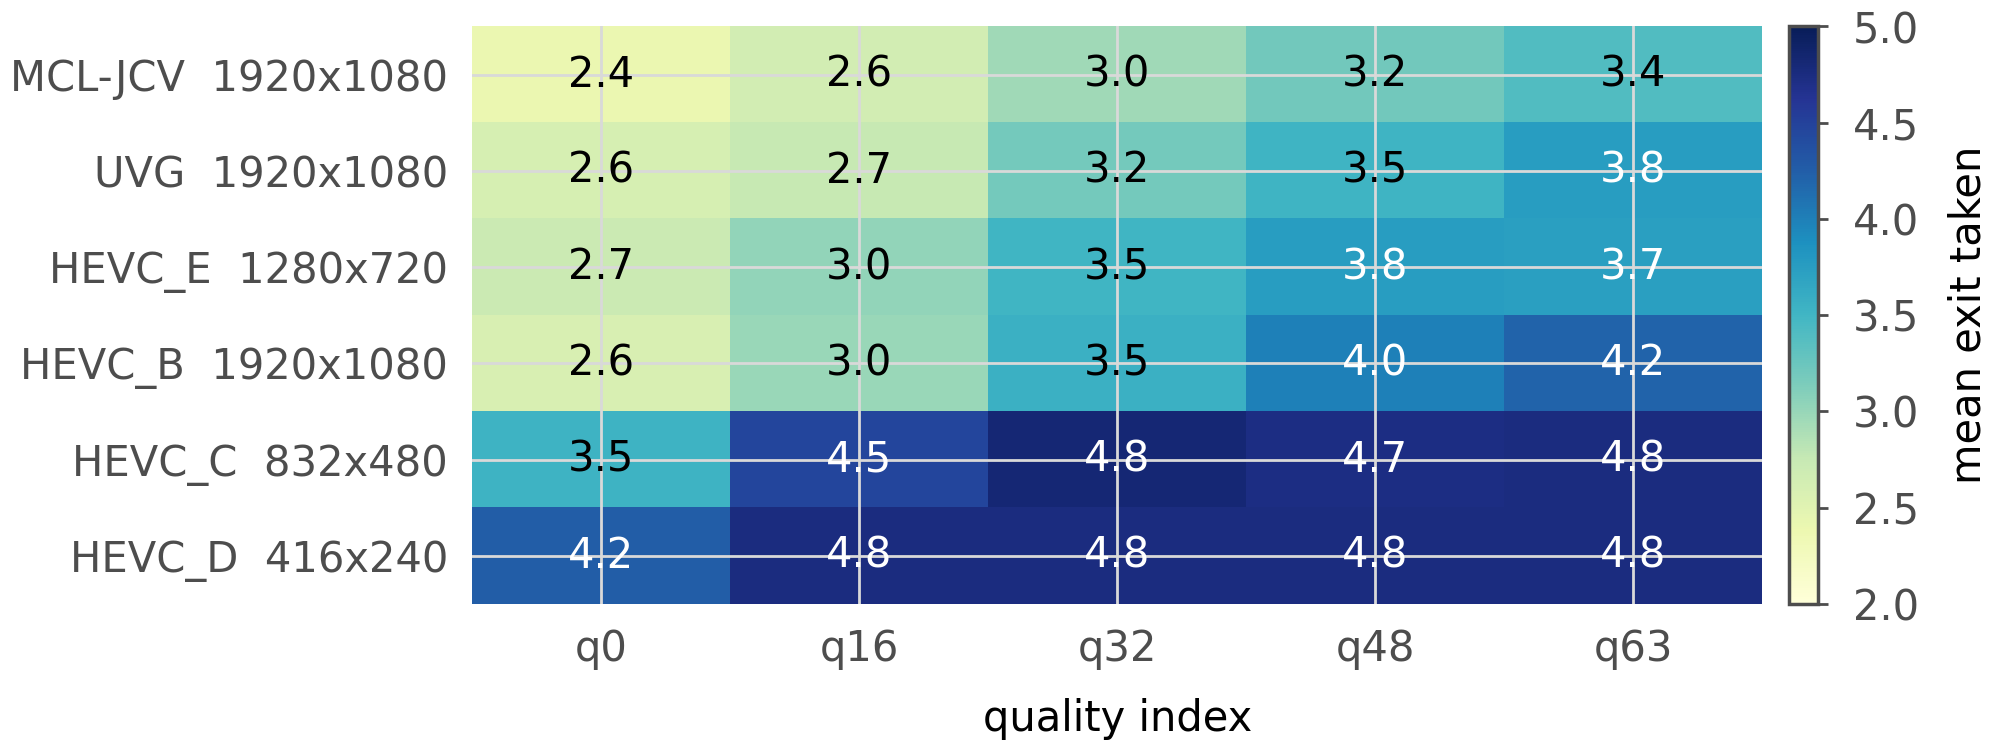
\includegraphics[width=\columnwidth]{figures/exituse.png}
\caption{\textbf{How deep each class has to go.} Mean exit taken by the tiles of each test class at the 0.1 dB budget, ordered by that mean. Resolution is the strongest predictor: the 416$\times$240 class has two tiles a frame and almost no choice, and the 1080p classes have forty and use the whole ladder. This is the dependence the main paper's tile-count section measures, seen per class rather than pooled.}
\end{figure}

\begin{figure}[t]
\centering
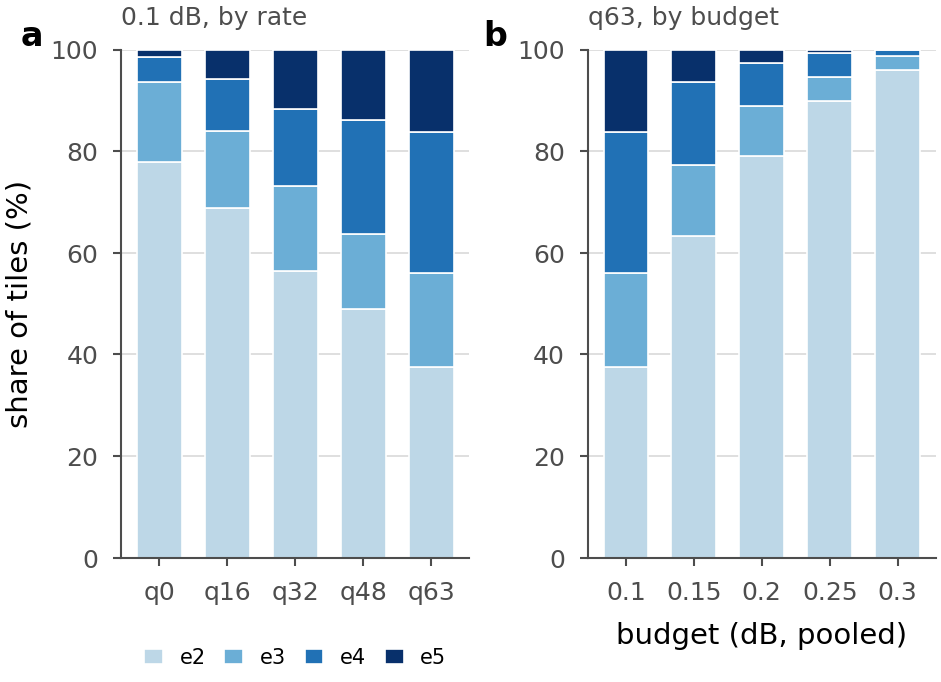
\includegraphics[width=\columnwidth]{figures/res_exits.png}
\caption{How the ladder fills up. \textbf{a}, exit shares at the 0.1 dB budget as the rate rises. \textbf{b}, exit shares at q63 as the budget loosens, until at 0.3 dB 96\% of tiles are already at the shallowest exit and there is almost nothing left to allocate. Both panels are pooled over the test set.}
\end{figure}

{\small Drawn by scripts/supp\_results\_figs.py from results/supp\_paper\_curve\_PAPER.json, on runs/RECIPE512/ckpt\_PAPER.pth.tar, pooled convention, so the budgets on the horizontal axis of \textbf{b} are looser than the identically labelled ones in the table above.}

\begin{table}[t]
\centering
\resizebox{\columnwidth}{!}{%
\begin{tabular}{lrrrrrrrr}
\toprule
Class & e2 & e3 & e4 & e5 & e2 & e3 & e4 & e5 \\
\midrule
MCL-JCV & 88.5 & 9.3 & 1.8 & 0.3 & 57.8 & 19.7 & 14.4 & 8.1 \\
UVG & 80.4 & 18.2 & 1.4 & 0.0 & 40.0 & 31.1 & 27.5 & 1.4 \\
HEVC B & 75.5 & 21.0 & 2.0 & 1.5 & 26.5 & 20.5 & 32.5 & 20.5 \\
HEVC E & 84.4 & 13.3 & 2.2 & 0.0 & 57.8 & 24.4 & 6.7 & 11.1 \\
HEVC C & 18.8 & 68.8 & 12.5 & 0.0 & 0.0 & 12.5 & 18.8 & 68.8 \\
HEVC D & 0.0 & 62.5 & 25.0 & 12.5 & 0.0 & 0.0 & 25.0 & 75.0 \\
\bottomrule
\end{tabular}}
\caption{The same histogram split by class at the two ends of the rate range: the first four columns are q0 and the second four are q63, each as a percentage of that class's tiles. HEVC C and HEVC D reach neither of the two shallowest exits at q63, and three quarters of their tiles run to full depth, which is the \SmallResHigh\% saving of the first table seen tile by tile. UVG behaves differently from MCL-JCV at q63 despite being the same resolution, which is content and not geometry.}
\end{table}

{\small results/supp\_per\_class\_budgets.json, on runs/RECIPE512/ckpt\_PAPER.pth.tar.}

\subsection{The frontier, class by class}

\begin{figure*}[t]
\centering
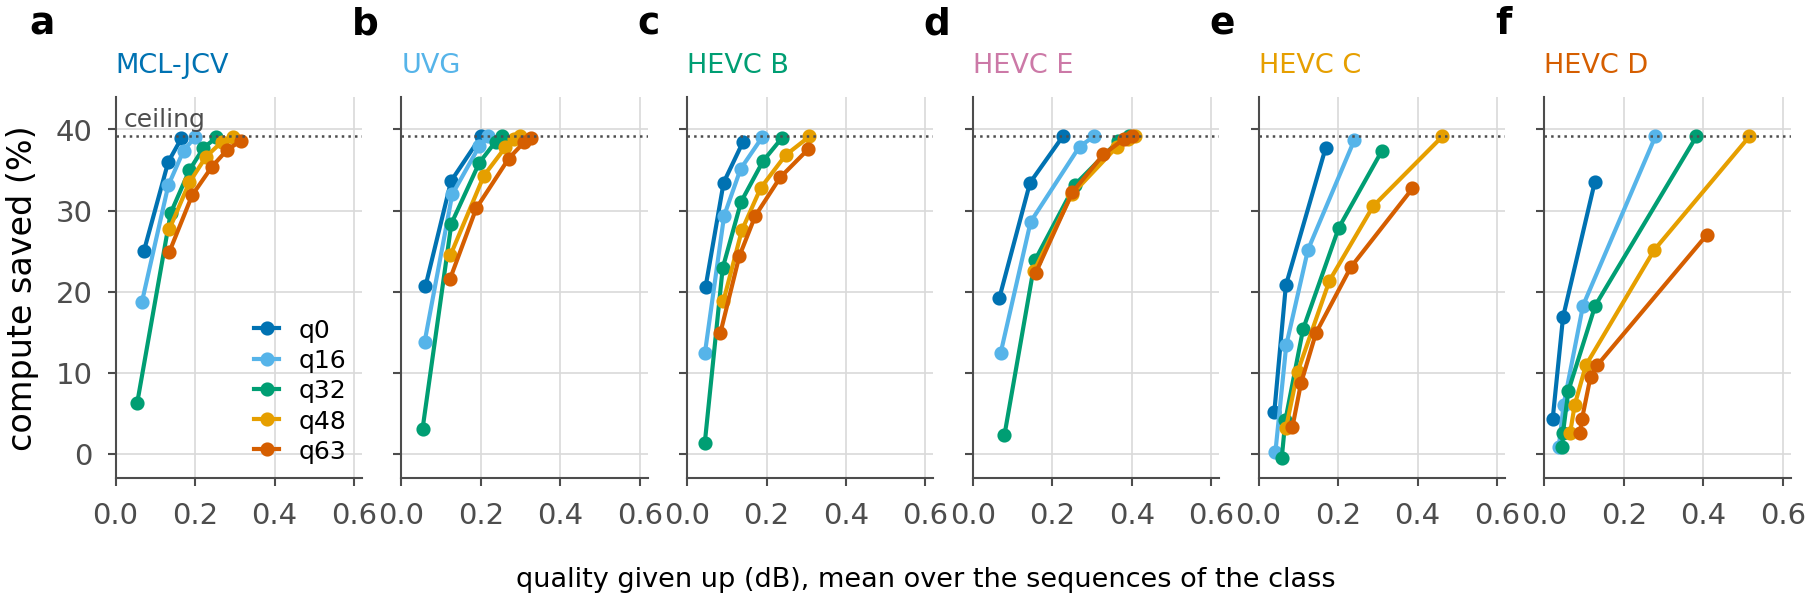
\includegraphics[width=\textwidth]{figures/res_frontier.png}
\caption{Compute saved against quality given up, one panel per class and one curve per quality index, from the seven budgets at which the frontier was measured. The dotted line is the architectural ceiling of \CeilingModelled\%. Three things are visible that a table of operating points hides. The curves are steep and then flat, so most of the saving is bought in the first tenth of a decibel and the rest of the band buys little. The rate ordering is preserved at every budget, so a curve never crosses another within a panel. And the panels move to the right as resolution falls: MCL-JCV reaches the ceiling by 0.3 dB at every rate, while HEVC D needs 0.5 dB at q48 and does not reach it at q63 within the measured range.}
\end{figure*}

{\small Drawn by scripts/supp\_results\_figs.py from results/supp\_paper\_curve\_PAPER.json, on runs/RECIPE512/ckpt\_PAPER.pth.tar. A point is the mean over the sequences of that class at a global operating point, so the multiplier is the one the whole set was bisected to and not a per-class retuning. Class membership per sequence from results/supp\_opquality\_PAPER.json, same checkpoint.}

Two limits bound every panel. A budget below the floor cannot be met at all, because our deepest exit already differs from the released decoder by \FloorLow dB at q0 and \FloorHigh dB at q63 in the per-frame convention; a budget above \SatLow dB at q0 or \SatHigh dB at q63 changes nothing, because every tile is already at the shallowest selectable exit. Between those two the multiplier is doing work, and the 0.1 dB budget is inside the window at every rate.

\subsection{Per-sequence spread}

A set mean is not what any single clip receives. One multiplier prices compute for the whole set, so each sequence lands wherever its own content puts it, and the spread of those landings is what a deployment would have to plan against.

\begin{table}[t]
\centering
\resizebox{\columnwidth}{!}{%
\begin{tabular}{lrrrrrrrr}
\toprule
Rate & n & Mean & SD & Min & p25 & Median & p75 & Max \\
\midrule
q0 & 53 & 36.8 & 3.7 & 24.2 & 35.8 & 38.8 & 39.1 & 39.1 \\
q16 & 53 & 33.1 & 8.1 & -1.0 & 30.4 & 36.1 & 38.8 & 39.1 \\
q32 & 53 & 29.5 & 10.2 & -1.0 & 26.1 & 32.6 & 37.6 & 39.1 \\
q48 & 53 & 27.9 & 10.7 & -1.0 & 23.2 & 31.1 & 36.5 & 39.1 \\
q63 & 53 & 26.7 & 10.8 & -1.0 & 22.6 & 29.9 & 34.3 & 39.1 \\
\bottomrule
\end{tabular}}
\caption{Compute saved per sequence at the 0.1 dB budget: the distribution behind the mean, over all \NumSeq sequences. The interquartile range widens from 9.9 points at q0 to 15.0 at q63, and the gap between best and worst sequence widens from 33.1 to 40.1. The minimum is negative at four of the five rates, because a sequence whose tiles all run to full depth costs 0.95\% more than the released decoder: our deepest exit is the more expensive of the two. Counting over rates as well as sequences, 15 of the 265 pairs save less than a tenth of a decode at this budget.}
\end{table}

{\small results/supp\_per\_sequence\_PAPER\_b010.json, on runs/RECIPE512/ckpt\_PAPER.pth.tar, read from its rows\_vs\_release block so that the denominator is the released decoder. Pooled convention, because the operating points come from results/supp\_paper\_curve\_PAPER.json.}

\begin{table}[t]
\centering
\resizebox{\columnwidth}{!}{%
\begin{tabular}{lrrr}
\toprule
Sequence & q0 & q63 & q63 dB \\
\midrule
BQSquare\_416x240 & 24.2 & -1.0 & 0.146 \\
RaceHorses\_416x240 & 24.2 & -1.0 & 0.064 \\
RaceHorses\_832x480 & 31.7 & 3.9 & 0.079 \\
PartyScene\_832x480 & 27.9 & 5.7 & 0.098 \\
BlowingBubbles\_416x240 & 31.7 & 6.0 & 0.072 \\
BasketballDrill\_832x480 & 30.3 & 7.4 & 0.001 \\
videoSRC27 & 39.1 & 39.1 & 0.127 \\
videoSRC29 & 39.1 & 39.1 & 0.126 \\
\bottomrule
\end{tabular}}
\caption{The six hardest sequences at q63 and the two easiest, with their q0 value beside them and the decibel each actually received. All six of the hard ones are 832x480 or 416x240. The delivered decibel is not the budget on any of them: across the \NumSeq sequences at q63 it runs from 0.013 dB to 0.237 dB against a 0.1 dB target, so a single multiplier for the set means some clips overshoot the budget by more than a factor of two while others use an eighth of it.}
\end{table}

{\small results/supp\_per\_sequence\_PAPER\_b010.json, on runs/RECIPE512/ckpt\_PAPER.pth.tar. Savings are against the released decoder; the decibel is the sequence's own, in the pooled convention.}

\subsection{A second metric, and the tiles that pay for the mean}

The whole mechanism is denominated in PSNR, and PSNR is known not to track visual quality closely. Two things follow that are worth measuring rather than asserting: whether a perceptual metric agrees that the loss is small, and how the loss is distributed over tiles, since a mean of 0.1 dB is compatible with a few tiles losing a great deal.

\begin{table}[t]
\centering
\resizebox{\columnwidth}{!}{%
\begin{tabular}{lrrrrrrr}
\toprule
Rate & bpp & PSNR & ours & lost & MS-SSIM & ours & lost \\
\midrule
q0 & 0.2314 & 32.536 & 32.435 & 0.1012 & 0.89934 & 0.89818 & 0.0498 \\
q16 & 0.2671 & 35.335 & 35.235 & 0.1003 & 0.94904 & 0.94855 & 0.0417 \\
q32 & 0.3351 & 38.135 & 38.036 & 0.0990 & 0.97565 & 0.97544 & 0.0375 \\
q48 & 0.4560 & 40.777 & 40.675 & 0.1014 & 0.98790 & 0.98780 & 0.0334 \\
q63 & 0.6716 & 43.155 & 43.044 & 0.1117 & 0.99419 & 0.99414 & 0.0390 \\
\bottomrule
\end{tabular}}
\caption{PSNR and MS-SSIM at the 0.1 dB operating point, over the whole test set. MS-SSIM agrees with PSNR about the direction and is kinder about the size: expressed as -10log10(1 minus MS-SSIM), the loss is 0.052 dB at q0 against 0.102 dB of PSNR, and 0.046 against 0.118 at q63, so on this metric the budget costs about half what the decibel it is written in suggests. Each metric is given as the released decoder, ours, and what was lost, with the MS-SSIM loss expressed as -10log10(1 minus MS-SSIM) so that the two loss columns are in the same unit. The bpp column is the released bitstream, which early exiting does not change beyond the exit map.}
\end{table}

{\small results/supp\_opquality\_PAPER.json, on runs/RECIPE512/ckpt\_PAPER.pth.tar, \NumSeq sequences at one frame each. MS-SSIM is Wang et al. 2003 at five scales with an 11-tap Gaussian of $\sigma$ = 1.5 on the valid region, on the luma plane in 4:2:0 on 0 to 255, the domain the PSNR column uses; the implementation self-checks at start-up and the file records that identical inputs score 1.000000 and a 3x3 box blur 0.7797. $\lambda$ is read from results/signalled\_RECIPE512\_ctc53.json so the allocation is the deployed one, and the delivered decibel recomputed here matches the stored value to four decimals.}

\begin{figure}[t]
\centering
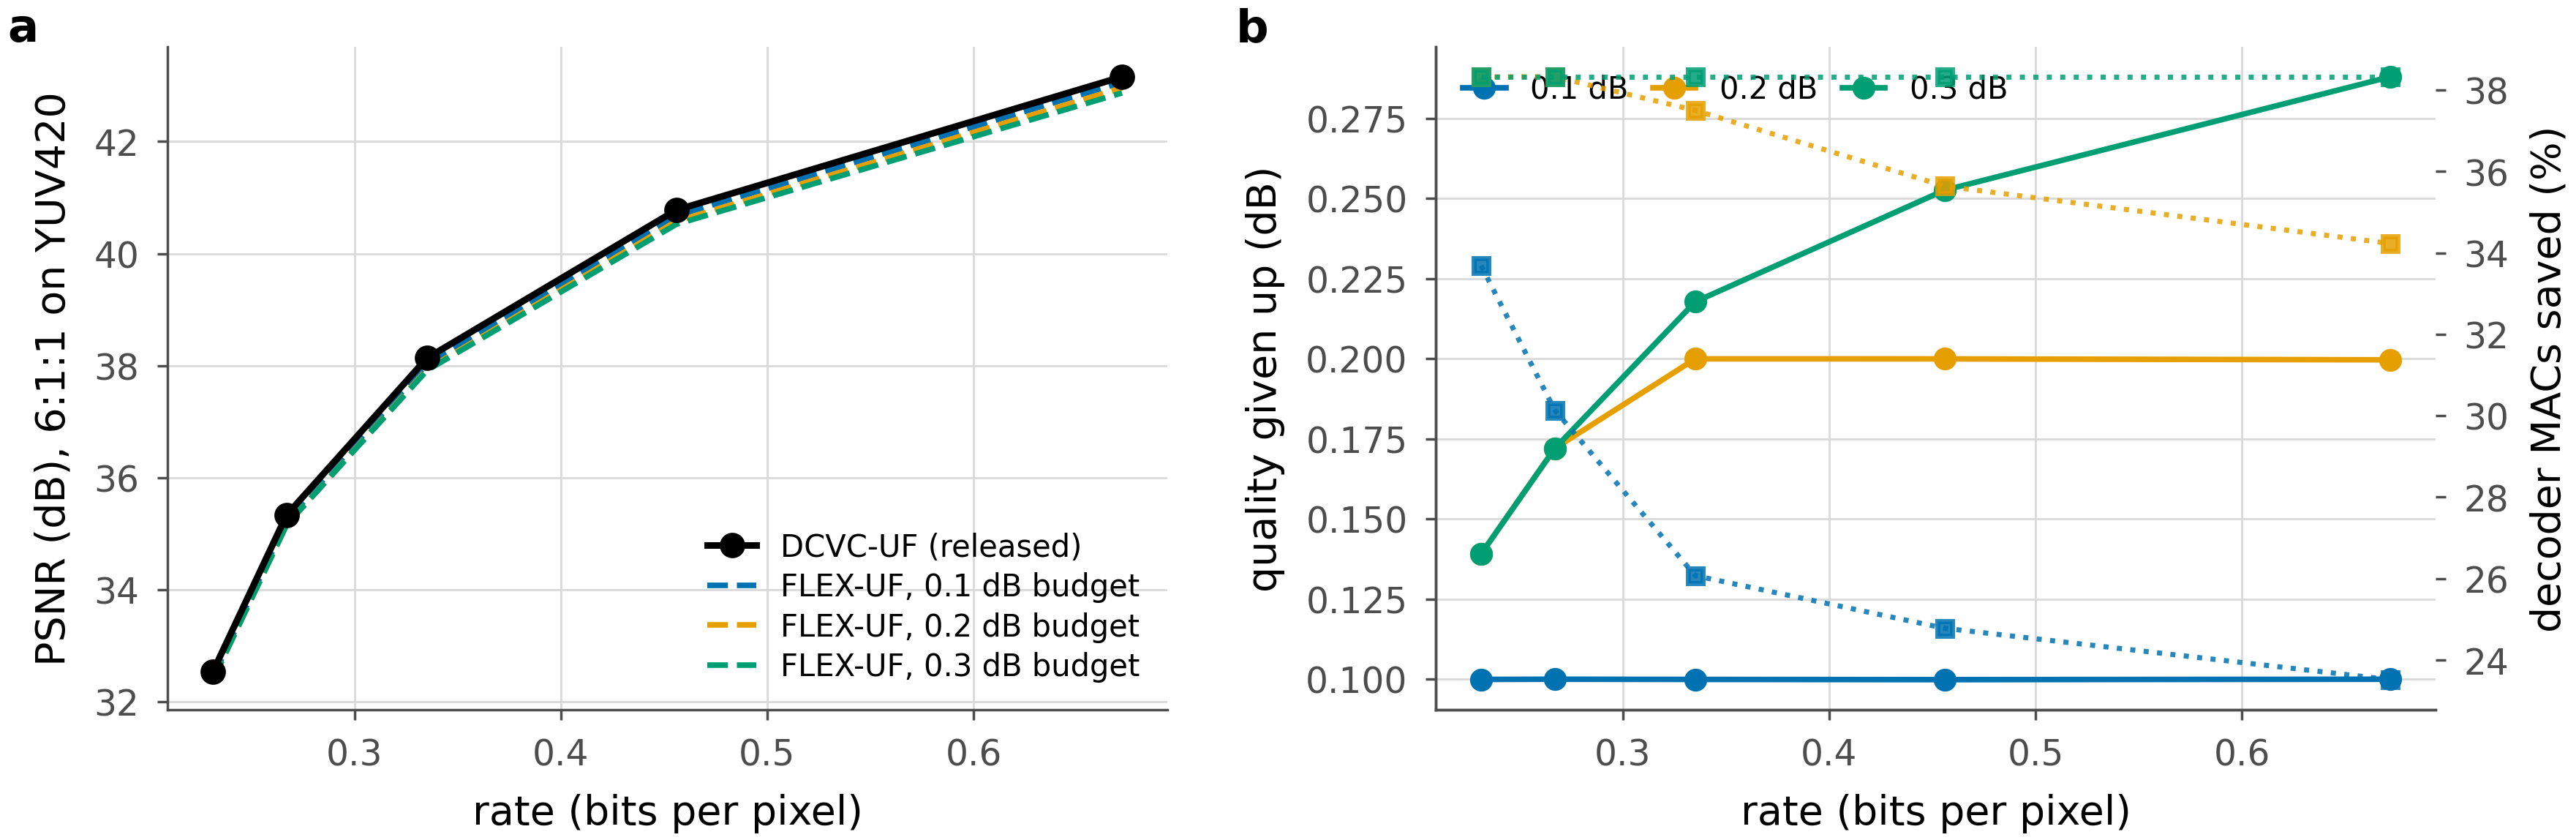
\includegraphics[width=\columnwidth]{figures/rd_vs_uf.png}
\caption{\textbf{a}, rate against quality over the five quality indices, the released DCVC-UF intra decoder and FLEX-UF at three budgets, on the \NumSeq CTC intra frames. Both axes come from one pass over the same frames, and the encoders are asserted bit-identical on the weights before a shared rate is reported, because a shared x-axis is a claim rather than a convenience. \textbf{b}, the same difference magnified: the decibels each budget delivered, against the decoder arithmetic it bought on the right-hand axis.}
\end{figure}

{\small Drawn by scripts/rd\_vs\_uf\_figure.py from results/rd\_absolute\_PAPER.json and results/signalled\_RECIPE512\_ctc53.json, both on runs/RECIPE512/ckpt\_PAPER.pth.tar.}

\begin{figure}[t]
\centering
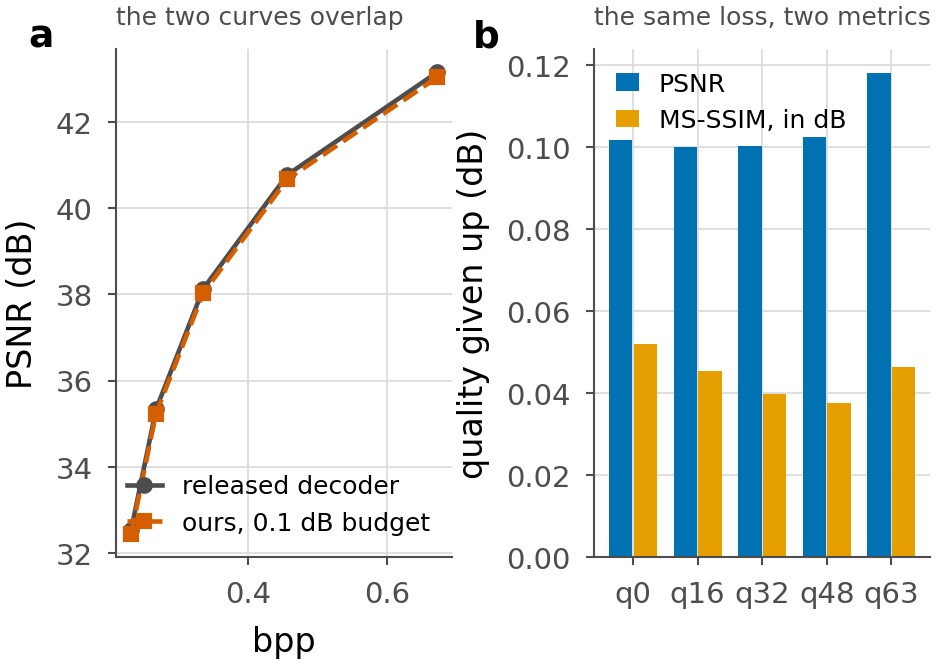
\includegraphics[width=\columnwidth]{figures/res_rd.png}
\caption{\textbf{a}, the rate-quality curve of the released decoder and of ours at the 0.1 dB budget, over the five quality indices. At plot scale they are one curve, which is what a 0.1 dB budget means. \textbf{b}, the gap that panel \textbf{a} cannot show, in PSNR and in MS-SSIM expressed as a decibel.}
\end{figure}

{\small Drawn by scripts/supp\_results\_figs.py from results/supp\_opquality\_PAPER.json, on runs/RECIPE512/ckpt\_PAPER.pth.tar.}

\begin{table}[t]
\centering
\resizebox{\columnwidth}{!}{%
\begin{tabular}{lrrrrrrrrr}
\toprule
Rate & Tiles & Mean & Median & p95 & p99 & Max & Over 0.25 & Over 0.5 & Over 1.0 \\
\midrule
q0 & 1765 & 0.145 & 0.106 & 0.429 & 0.945 & 1.379 & 244 & 66 & 15 \\
q16 & 1765 & 0.139 & 0.109 & 0.388 & 0.660 & 1.299 & 211 & 50 & 5 \\
q32 & 1765 & 0.141 & 0.107 & 0.393 & 0.640 & 1.032 & 218 & 48 & 1 \\
q48 & 1765 & 0.140 & 0.109 & 0.374 & 0.722 & 1.423 & 191 & 47 & 4 \\
q63 & 1765 & 0.139 & 0.106 & 0.386 & 0.744 & 1.421 & 195 & 48 & 4 \\
\bottomrule
\end{tabular}}
\caption{How the 0.1 dB is distributed over the 1765 tiles of one pass over the test set. The last three columns count tiles losing more than a quarter, a half and a whole decibel. The median tile is at or below the budget at every rate, and the tail is long: at q0, 302 tiles lose more than 0.25 dB, 79 lose more than 0.5 dB, and the worst loses 1.97 dB. A budget stated as a mean says nothing about the last three columns, which is why they are printed.}
\end{table}

{\small results/supp\_opquality\_PAPER.json, on runs/RECIPE512/ckpt\_PAPER.pth.tar, at the same operating points as the metric table above. A tile penalty is the decibel between the released decode of that tile and ours.}

\begin{figure}[t]
\centering
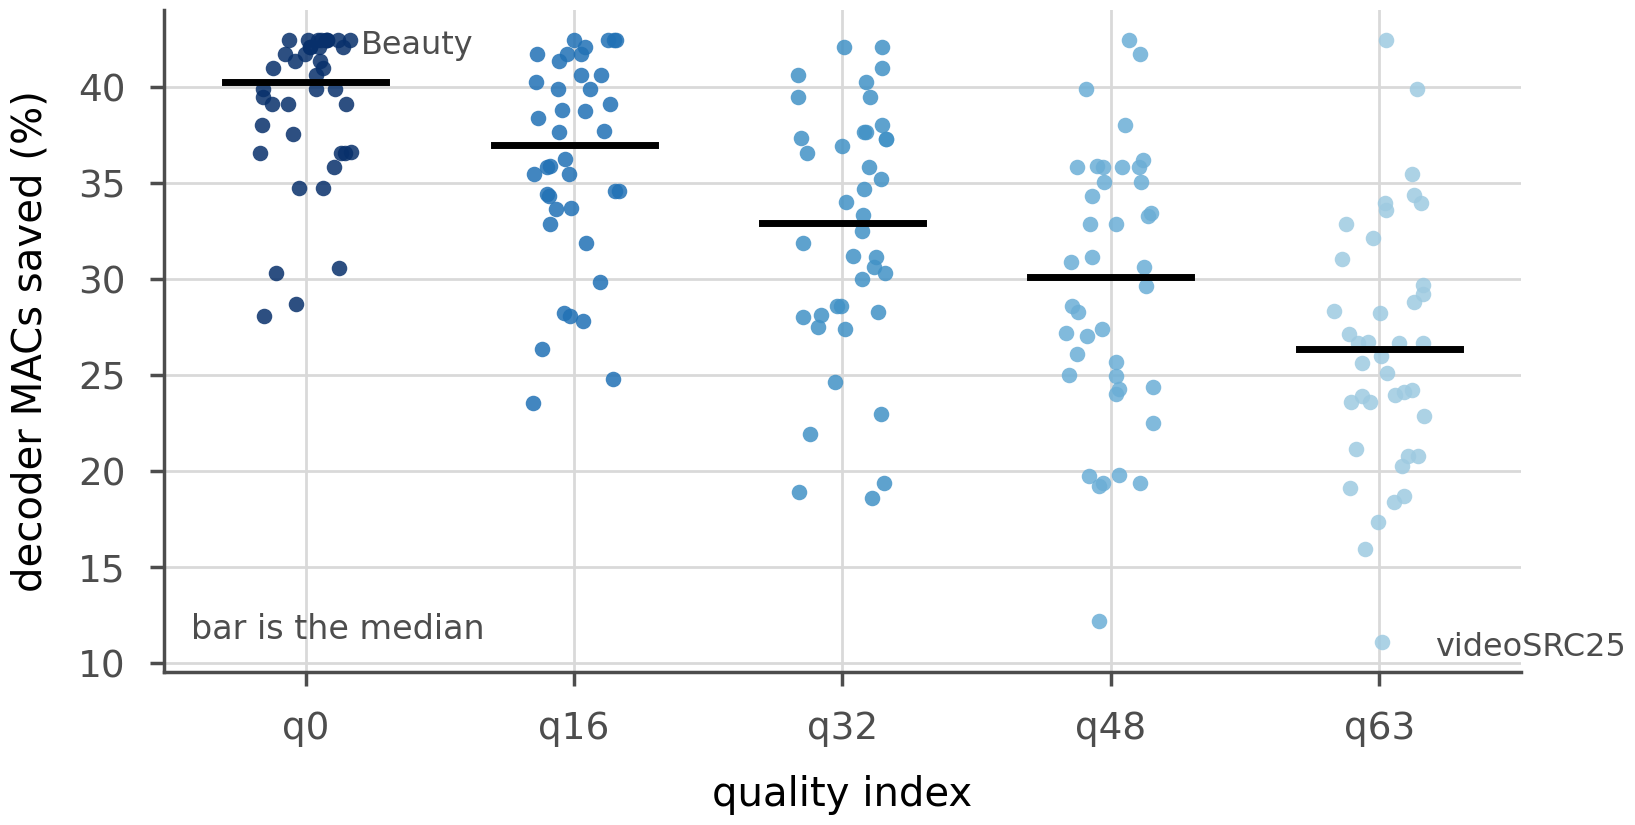
\includegraphics[width=\columnwidth]{figures/spread.png}
\caption{\textbf{What the set mean hides.} Every test sequence as a point, at the 0.1 dB budget; the bar is the median. At the lowest rate the saving runs from \SpreadLowMin\% to \SpreadLowMax\% across the \SpreadNSeq sequences and at the highest from \SpreadHighMin\% to \SpreadHighMax\%. The spread within a rate is larger than the difference between rates, and it is content, not noise: the same sequences sit at the same end of it at every rate. }
\end{figure}

\begin{figure}[t]
\centering
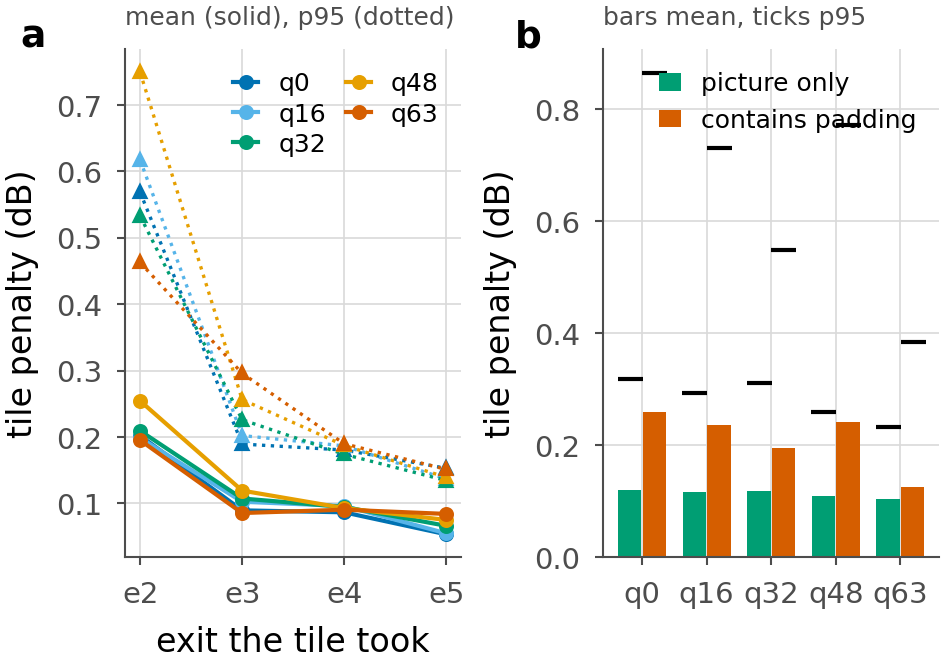
\includegraphics[width=\columnwidth]{figures/res_tail.png}
\caption{Where the tail comes from. \textbf{a}, mean and 95th percentile tile penalty against the exit the tile took. The tail sits on e2, the shallowest exit the clamp allows: at q0 its mean is 0.202 dB against 0.054 dB at e5, and all 79 tiles above 0.5 dB took it. \textbf{b}, the same penalty split by whether the tile contains replicated padding. A 1080p frame is padded to 2048x1280, so 200 of the bottom tile row's 256 rows are invented by replication, and those tiles carry roughly double the mean penalty at every rate: 0.261 dB against 0.121 dB at q0, and 65 of the 79 tiles above half a decibel are padded ones.}
\end{figure}

{\small Drawn by scripts/supp\_results\_figs.py from the tail\_by\_exit and tail\_by\_padding blocks of results/supp\_opquality\_PAPER.json, on runs/RECIPE512/ckpt\_PAPER.pth.tar. A tile counts as padded if any of its pixels came from the replicate pad, recorded per tile as pad\_fraction. Padding geometry from results/tile\_definition.json, same checkpoint.}

\subsection{Composition with weight quantisation}

Early exiting removes work and quantisation makes the remaining work cheaper, so the two ought to compose. Whether they do is a question about the same weights, and it is measured here rather than assumed.

\begin{table}[t]
\centering
\resizebox{\columnwidth}{!}{%
\begin{tabular}{lrrrrrr}
\toprule
Weights & Rate & e2 & e3 & e4 & e5 & Layers \\
\midrule
float32 & q0 & 0.132 & 0.058 & 0.039 & 0.021 & 0 \\
float32 & q32 & 0.284 & 0.144 & 0.100 & 0.037 & 0 \\
float32 & q63 & 0.650 & 0.371 & 0.265 & 0.085 & 0 \\
int8 & q0 & 0.140 & 0.065 & 0.045 & 0.026 & 86 \\
int8 & q32 & 0.315 & 0.171 & 0.129 & 0.062 & 86 \\
int8 & q63 & 0.776 & 0.496 & 0.394 & 0.207 & 86 \\
int6 & q0 & 0.297 & 0.217 & 0.206 & 0.169 & 86 \\
int6 & q32 & 1.046 & 0.877 & 0.845 & 0.736 & 86 \\
int6 & q63 & 2.794 & 2.535 & 2.506 & 2.287 & 86 \\
int4 & q0 & 1.835 & 1.594 & 1.555 & 1.390 & 86 \\
int4 & q32 & 4.390 & 4.120 & 4.138 & 3.907 & 86 \\
int4 & q63 & 8.356 & 8.039 & 8.139 & 7.898 & 86 \\
\bottomrule
\end{tabular}}
\caption{Quality given up against the released decoder with the decoder weights quantised, at four exits and three rates. The float32 rows are the ladder itself and are the baseline each integer row should be read against. At q0 int8 is nearly free, moving the deepest exit from 0.027 dB to 0.032 dB, so the two levers compose. At q63 they compete: the deepest exit moves from 0.108 dB to 0.223 dB, which is more than a whole 0.1 dB budget spent before any tile has exited early. Six-bit costs 0.13 dB at the deepest exit at q0 and 2.18 dB at q63, and four-bit is unusable at every rate. The last column is the number of layers quantised, the same 86 in every integer row.}
\end{table}

{\small results/supp\_quant\_PAPER.json, on runs/RECIPE512/ckpt\_PAPER.pth.tar, 32 held-out images at 512 px. Weight-only, symmetric, per output channel, no calibration, on dec.* and router\_head.* with the encoder asserted unchanged. Nothing here measures an integer kernel: the file records the bit width and the implied bit-operation ratio, and the arithmetic ran in floating point on quantised weights.}

\subsection{Integrated figures, and what they depend on}

A budget is one sample of a curve. Video coding answers this for rate against quality with Bjontegaard's construction [4], integrating one axis over a stated interval of the other, and the same construction applies with compute in place of rate. BD-saving is the mean compute saved over an interval of decibels and BD-quality is the mean decibel paid over an interval of saving. Neither means anything without its interval and its convention, and both are given with theirs.

\begin{table}[t]
\centering
\resizebox{\columnwidth}{!}{%
\begin{tabular}{lrrrrr}
\toprule
Rate & BD-saving & BD-quality & BD-saving & BD-quality & Points \\
\midrule
q0 & 33.2\% & 0.0372 & 34.9\% & 0.0330 & 15 \\
q16 & 29.4\% & 0.0509 & 31.6\% & 0.0437 & 14 \\
q32 & 24.8\% & 0.0652 & 27.7\% & 0.0544 & 13 \\
q48 & 23.0\% & 0.0705 & 25.7\% & 0.0595 & 13 \\
q63 & 20.9\% & 0.0758 & 24.0\% & 0.0636 & 12 \\
Mean where defined & 26.3\% & 0.0599 & 28.8\% & 0.0508 &  \\
\bottomrule
\end{tabular}}
\caption{BD-saving and BD-quality per rate under both decibel conventions: the first pair of columns is per frame and the second is pooled. BD-saving is defined at only two of the five rates, because at q0, q16 and q32 the frontier saturates below the upper limit of the interval and there is no curve left to integrate. The convention moves the answer by 1.9 points of BD-saving and 0.018 dB of BD-quality on identical allocations, and it moves it consistently, since per-frame averaging raises every floor and pooling does not. Points is the number of measured frontier points inside the interval.}
\end{table}

{\small results/supp\_bd\_PAPER\_per\_frame.json and results/supp\_bd\_PAPER\_pooled.json, both on runs/RECIPE512/ckpt\_PAPER.pth.tar over \NumSeq sequences, integrating results/supp\_paper\_curve\_PAPER.json. BD-saving is over 0.066 to 0.300 dB per frame and 0.059 to 0.300 dB pooled, the lower limit being the highest floor any rate has under that convention. BD-quality is over 10\% to 30\% saving. The floors that set those lower limits are recorded per rate in both files as floor\_db, and appear directly in the frontier table below at the two rates where the 0.05 dB budget is unreachable.}

Two sensitivities sit around those numbers and are worth stating beside them. The first is the anchor. Our deepest exit is not bit-exact with the released decoder, since it carries seam repair and a fine-tuned trunk, and it starts every budget slightly behind: the drift runs from 0.005 dB at q0 to 0.036 dB at q63, which at q63 is a third of the whole budget. Setting it to zero would raise BD-saving at q63 from 28.7\% to 34.9\%, a gain of 6.2 points. The second is the interval. Over six defensible intervals the mean BD-saving moves from 22.8\% to 29.2\%, a range of 6.3 points, while the gap between the lowest and highest rate stays inside 15.3 to 16.8 points on every one of them; the level depends on the integration and the rate effect does not.

{\small Anchor drift from results/supp\_anchor\_PAPER.json, on runs/RECIPE512/ckpt\_PAPER.pth.tar, \NumSeq frames, per-frame convention; the zero-drift figure is the bd\_saving\_pct\_zero\_drift field of results/supp\_bd\_PAPER\_per\_frame.json. Interval sensitivity from results/bd\_sensitivity.json, which is not pinned: scripts/bd\_sensitivity.py names its curve as results/paper\_curve\_grid128.json, on runs/wdec\_j2\_p128\_grid/ckpt\_epo0.pth.tar at 128 px tiles over 40 sequences, so its levels are not the levels above and only its robustness conclusion is quoted.}

\begin{table}[t]
\centering
\resizebox{\columnwidth}{!}{%
\begin{tabular}{lrrrrr}
\toprule
Budget & A BD-Rate & B BD-Rate & Difference & A saved & B saved \\
\midrule
0.1 dB & 1.032\% & 1.007\% & 0.025 pt & 28.3\% & 25.3\% \\
0.3 dB & 2.339\% & 2.318\% & 0.020 pt & 39.1\% & 39.0\% \\
0.5 dB & 2.339\% & 2.318\% & 0.020 pt & 39.1\% & 39.0\% \\
\bottomrule
\end{tabular}}
\caption{BD-Rate cost of the two configurations: the rate a reader would have to spend to buy back the quality the compute saving costs, integrated over the five rate points, which is the number that makes this trade-off comparable with a published codec result. Configuration A signals the exit map in the bitstream and pays \MapBitsLo to \MapBitsHi bits a frame for it at the 0.1 dB budget, depending on the rate, configuration B infers it from what the decoder already holds and pays none. Their BD-Rate costs differ by at most 0.025 of a point, so the map is close to free. What A buys with it is compute: the gap in the last two columns is 3.0 points at the tight budget and 0.2 at the loose one, where both configurations are at the ceiling.}
\end{table}

{\small results/bdrate.json, every row on runs/RECIPE512/ckpt\_PAPER.pth.tar, which its sources block records file by file.}

\subsection{Raw values behind the curves}

Everything above is an integral, a mean or a picture. What follows is the measured numbers themselves, so that a reader can compare against them without digitising a plot or rerunning a decode.

\begin{table}[t]
\centering
\resizebox{\columnwidth}{!}{%
\begin{tabular}{lrrrrrr}
\toprule
Rate & Budget & lambda & dB & Model & Meter & Map bits \\
\midrule
q0 & 0.1 & 7.280e-05 & 0.0999 & 34.5 & 33.7 & 64 \\
q0 & 0.2 & 1.000e+00 & 0.1391 & 39.1 & 38.3 & 48 \\
q0 & 0.3 & 1.000e+00 & 0.1391 & 39.1 & 38.3 & 48 \\
q0 & 0.5 & 1.000e+00 & 0.1391 & 39.1 & 38.3 & 48 \\
q16 & 0.1 & 2.912e-05 & 0.1000 & 30.8 & 30.1 & 75 \\
q16 & 0.2 & 1.000e+00 & 0.1720 & 39.1 & 38.3 & 48 \\
q16 & 0.3 & 1.000e+00 & 0.1720 & 39.1 & 38.3 & 48 \\
q16 & 0.5 & 1.000e+00 & 0.1720 & 39.1 & 38.3 & 48 \\
q32 & 0.1 & 1.305e-05 & 0.0999 & 26.7 & 26.1 & 84 \\
q32 & 0.2 & 8.293e-05 & 0.2000 & 38.3 & 37.5 & 52 \\
q32 & 0.3 & 1.000e+00 & 0.2178 & 39.1 & 38.3 & 48 \\
q32 & 0.5 & 1.000e+00 & 0.2178 & 39.1 & 38.3 & 48 \\
q48 & 0.1 & 7.315e-06 & 0.0999 & 25.4 & 24.8 & 89 \\
q48 & 0.2 & 3.485e-05 & 0.2000 & 36.4 & 35.6 & 57 \\
q48 & 0.3 & 1.000e+00 & 0.2526 & 39.1 & 38.3 & 48 \\
q48 & 0.5 & 1.000e+00 & 0.2526 & 39.1 & 38.3 & 48 \\
q63 & 0.1 & 4.534e-06 & 0.1000 & 24.1 & 23.5 & 91 \\
q63 & 0.2 & 1.972e-05 & 0.1997 & 35.0 & 34.2 & 61 \\
q63 & 0.3 & 1.000e+00 & 0.2880 & 39.1 & 38.3 & 48 \\
q63 & 0.5 & 1.000e+00 & 0.2880 & 39.1 & 38.3 & 48 \\
\bottomrule
\end{tabular}}
\caption{The deployed operating points: four budgets at five rates. Model is the saving the cost model predicts for the chosen map and Meter is what a forward hook on every convolution and linear layer counted on the same decode, so the two columns are the cost model checked against itself; the model reads high by 0.4 to 0.8 points throughout. Map bits is the entropy of the per-frame exit histogram, charged to the bitstream before any saving is computed, and it falls as the budget loosens because the histogram concentrates.}
\end{table}

{\small results/signalled\_RECIPE512\_ctc53.json, on runs/RECIPE512/ckpt\_PAPER.pth.tar, \NumSeq sequences, per-frame convention. $\lambda$ is the multiplier the two-level bisection settled on, and a $\lambda$ of exactly 1 is the top of its bracket, which marks a budget the ladder saturated below rather than a price that was chosen. Saving is against the released decoder.}

\begin{table}[t]
\centering
\resizebox{\columnwidth}{!}{%
\begin{tabular}{lrrrrrr}
\toprule
Rate & Budget & lambda & dB pooled & dB per frame & Saved & e2/e3/e4/e5 \\
\midrule
q0 & 0.05 & 2.742e-05 & 0.0500 & 0.0611 & 29.0 & 51/31/11/6 \\
q0 & 0.1 & 1.077e-04 & 0.1000 & 0.1157 & 37.8 & 92/7/1/0 \\
q0 & 0.15 & n/a & 0.1239 & 0.1391 & 39.1 & 100/0/0/0 \\
q0 & 0.2 & n/a & 0.1239 & 0.1391 & 39.1 & 100/0/0/0 \\
q0 & 0.25 & n/a & 0.1239 & 0.1391 & 39.1 & 100/0/0/0 \\
q0 & 0.3 & n/a & 0.1239 & 0.1391 & 39.1 & 100/0/0/0 \\
q0 & 0.5 & n/a & 0.1239 & 0.1391 & 39.1 & 100/0/0/0 \\
q16 & 0.05 & 1.019e-05 & 0.0500 & 0.0605 & 24.3 & 40/28/15/17 \\
q16 & 0.1 & 4.165e-05 & 0.0999 & 0.1148 & 35.4 & 80/15/3/2 \\
q16 & 0.15 & 1.336e-04 & 0.1500 & 0.1646 & 38.9 & 98/2/0/0 \\
q16 & 0.2 & n/a & 0.1585 & 0.1720 & 39.1 & 100/0/0/0 \\
q16 & 0.25 & n/a & 0.1585 & 0.1720 & 39.1 & 100/0/0/0 \\
q16 & 0.3 & n/a & 0.1585 & 0.1720 & 39.1 & 100/0/0/0 \\
q16 & 0.5 & n/a & 0.1585 & 0.1720 & 39.1 & 100/0/0/0 \\
q32 & 0.05 & 4.037e-06 & 0.0500 & 0.0608 & 18.6 & 25/26/21/28 \\
q32 & 0.1 & 1.772e-05 & 0.1000 & 0.1157 & 32.5 & 69/18/8/4 \\
q32 & 0.15 & 4.134e-05 & 0.1500 & 0.1647 & 37.2 & 89/9/2/0 \\
q32 & 0.2 & 1.435e-04 & 0.1998 & 0.2152 & 39.1 & 100/0/0/0 \\
q32 & 0.25 & n/a & 0.2019 & 0.2178 & 39.1 & 100/0/0/0 \\
q32 & 0.3 & n/a & 0.2019 & 0.2178 & 39.1 & 100/0/0/0 \\
q32 & 0.5 & n/a & 0.2019 & 0.2178 & 39.1 & 100/0/0/0 \\
q48 & 0.05 & 1.884e-06 & 0.0500 & 0.0599 & 15.8 & 22/18/24/35 \\
q48 & 0.1 & 9.772e-06 & 0.1000 & 0.1148 & 31.0 & 64/19/12/6 \\
q48 & 0.15 & 2.126e-05 & 0.1500 & 0.1666 & 36.1 & 84/11/4/1 \\
q48 & 0.2 & 5.103e-05 & 0.1999 & 0.2191 & 38.5 & 96/3/1/0 \\
q48 & 0.25 & n/a & 0.2305 & 0.2526 & 39.1 & 100/0/0/0 \\
q48 & 0.3 & n/a & 0.2305 & 0.2526 & 39.1 & 100/0/0/0 \\
q48 & 0.5 & n/a & 0.2305 & 0.2526 & 39.1 & 100/0/0/0 \\
q63 & 0.05 & 1.054e-06 & 0.0500 & 0.0598 & 13.7 & 16/18/25/40 \\
q63 & 0.1 & 6.072e-06 & 0.1000 & 0.1154 & 29.7 & 58/21/15/6 \\
q63 & 0.15 & 1.282e-05 & 0.1499 & 0.1658 & 35.1 & 80/12/6/2 \\
q63 & 0.2 & 2.536e-05 & 0.1998 & 0.2180 & 37.8 & 93/6/2/0 \\
q63 & 0.25 & 6.566e-05 & 0.2498 & 0.2784 & 39.0 & 99/1/0/0 \\
q63 & 0.3 & n/a & 0.2613 & 0.2880 & 39.1 & 100/0/0/0 \\
q63 & 0.5 & n/a & 0.2613 & 0.2880 & 39.1 & 100/0/0/0 \\
\bottomrule
\end{tabular}}
\caption{The frontier itself: every operating point behind the per-class figure, at seven budgets and five rates, with the exit shares that produced each one. Both decibel conventions are printed for the same allocation, and they differ by 0.010 to 0.029 dB over the table and by 0.015 to 0.016 dB at the 0.1 dB budget, which is a fifth of that budget. A row reading n/a in the saving column is a budget below the floor at that rate, where no allocation meets the target. A row reading 100/0/0/0 is past saturation: the file stores neither a multiplier nor a histogram there, and the shares are filled in from what saturation means, every tile at the shallowest selectable exit.}
\end{table}

{\small results/supp\_paper\_curve\_PAPER.json, on runs/RECIPE512/ckpt\_PAPER.pth.tar. Saving is converted to the released-decoder denominator by charging the retained cost the price of our deepest exit, 1.0095 released decodes, which is \DeepestUniformCost at the precision the paper prints and is derived here from the ceiling in results/saturation\_RECIPE512\_ctc53.json and the saturated saving in this file. One caution about that denominator: this file bills the shared stem inside every tile's cost, while results/supp\_latency\_batch\_1920x1080.json bills it once per frame through flexuf/cost.py frame\_relative\_cost, and the two accountings differ by about a third of a point on an identical exit map at q0.}

\subsection{Reusing an exit map}

The signalled configuration pays one extra decode per frame at the encoder to find its map. How much that matters depends on how often the map has to be found again, so we probed two kinds of reuse: across frames of one sequence, and across the quality index. The probe is narrow and is reported as one.

\begin{table}[t]
\centering
\resizebox{\columnwidth}{!}{%
\begin{tabular}{lrrrrrr}
\toprule
reuse & map found at & applied at & in place, dB & reused, dB & in place, saved \% & reused, saved \% \\
\midrule
frames & q0 frame 0 & frame 1 & 0.0998 & 0.1014 & 34.20 & 34.20 \\
frames & q0 frame 0 & frame 2 & 0.0991 & 0.0994 & 34.40 & 34.20 \\
frames & q0 frame 0 & frame 4 & 0.0991 & 0.1007 & 34.40 & 34.20 \\
frames & q0 frame 0 & frame 8 & 0.0997 & 0.1024 & 34.52 & 34.20 \\
frames & q32 frame 0 & frame 1 & 0.0976 & 0.1012 & 30.43 & 30.89 \\
frames & q32 frame 0 & frame 2 & 0.0955 & 0.0992 & 30.66 & 30.89 \\
frames & q32 frame 0 & frame 4 & 0.0957 & 0.0970 & 30.94 & 30.89 \\
frames & q32 frame 0 & frame 8 & 0.0999 & 0.0976 & 31.76 & 30.89 \\
frames & q63 frame 0 & frame 1 & 0.0905 & 0.0930 & 26.35 & 26.46 \\
frames & q63 frame 0 & frame 2 & 0.0905 & 0.0933 & 26.24 & 26.46 \\
frames & q63 frame 0 & frame 4 & 0.0916 & 0.0939 & 26.33 & 26.46 \\
frames & q63 frame 0 & frame 8 & 0.0926 & 0.0934 & 26.71 & 26.46 \\
rate & q0 & q32 & 0.0982 & 0.1276 & 30.89 & 34.20 \\
rate & q0 & q63 & 0.0925 & 0.1586 & 26.46 & 34.20 \\
rate & q32 & q0 & 0.0998 & 0.0947 & 34.20 & 30.89 \\
rate & q32 & q63 & 0.0925 & 0.1228 & 26.46 & 30.89 \\
rate & q63 & q0 & 0.0998 & 0.0824 & 34.20 & 26.46 \\
rate & q63 & q32 & 0.0982 & 0.0874 & 30.89 & 26.46 \\
\bottomrule
\end{tabular}}
\caption{\textbf{What a reused exit map delivers.} Each row applies a map found in one place to a decode somewhere else and reports what that decode actually delivered, beside the map recomputed in place. Read the two decibel columns first: a reused map is only usable if the decode it produces still meets the budget, and the saving column means nothing on a row where it does not.}
\end{table}

{\small results/map\_transfer.json, budget 0.1 dB, on the checkpoint the file records. The offsets and the quality pairs in the file are the whole of the probe; nothing here is a statement about reuse in general.}

Across frames of one sequence, reuse is close to free. Taking the map found on frame 0 and applying it eight frames later raises the delivered distortion by \TransferDbCost dB at q0, about five percent of the budget, and the saving does not move at all: \TransferSaving\% transferred against \TransferInPlaceLo--\TransferInPlaceHi\% recomputed. The allocation is a property of where the content is hard, and that moves slowly. An encoder that searched once per group of pictures rather than once per frame would divide its extra cost by the group length, on the offsets we probed.

Across the quality index the map does have to be recomputed, and the direction decides how badly. Found at q0 and applied at q63 it delivers \TransferCrossDb dB against a 0.1 dB budget, claiming the low-rate saving of \TransferSaving\% while spending nearly twice the quality it is allowed. The reverse is safe and wasteful. Shallow exits are cheap in quality at low rate and expensive at high rate, so a map is calibrated to the rate it was found at, and reusing one upward breaks the quality guarantee with nothing in the decode reporting that it has. In our reuse probe, then, an encoder can search once per rate and reuse that search across the frames we tested; how far that carries beyond the offsets and sequences probed here we have not measured.

\subsection{Failure cases}

Five cases are worth naming, all of them measured in the files above rather than inferred.

\begin{itemize}\itemsep1pt
\item \textbf{Sequences that cost more than they save.} At q63 four sequences finish at minus 0.95\%, which is every tile at full depth and our deepest exit costing that much more than a released decode: RaceHorses at 832x480 and at 416x240, BlowingBubbles and BQSquare. One more sits under 3\% and ten in all save less than a tenth of a decode. On this content the method should be switched off rather than run at a budget, and the exit histogram is what tells the encoder so.
\item \textbf{The bottom tile row of a padded frame.} The six worst tiles in the test set are all in the last row of a 1080p frame at 78\% padding, each losing between 1.72 and 1.97 dB. The allocation is behaving correctly given its table, and the table is measuring a region that will be cropped away before anyone looks at it, so the budget is being spent on invented pixels.
\item \textbf{The two smallest classes at high rate.} HEVC C and HEVC D save \SmallResHigh\% at q63, which is one tile in four moved one exit up and nothing else. With two tiles on a 416x240 frame there is no allocation worth making, and the honest reading is that this method needs a frame large enough to hold a useful number of tiles.
\item \textbf{Quantisation and early exit compete at high rate.} Int8 weights cost 0.115 dB at q63 at the deepest exit, more than the whole budget the allocation is then asked to work inside, while at q0 they cost 0.005 dB. A deployment cannot assume the two savings multiply.
\item \textbf{A 0.5 dB budget has no per-sequence breakdown to report.} At 0.5 dB every rate is past saturation, the frontier stops at the ceiling of \CeilingModelled\%, and a saturated operating point carries no allocation to break down, which is why the per-sequence sweep runs from 0.10 dB to 0.30 dB.
\end{itemize}

{\small Worst tiles from the worst\_tiles block of results/supp\_opquality\_PAPER.json and negative sequences from results/supp\_per\_sequence\_PAPER\_b010.json, both on runs/RECIPE512/ckpt\_PAPER.pth.tar; the saturation points from results/saturation\_RECIPE512\_ctc53.json.}

\begin{figure}[t]
\centering
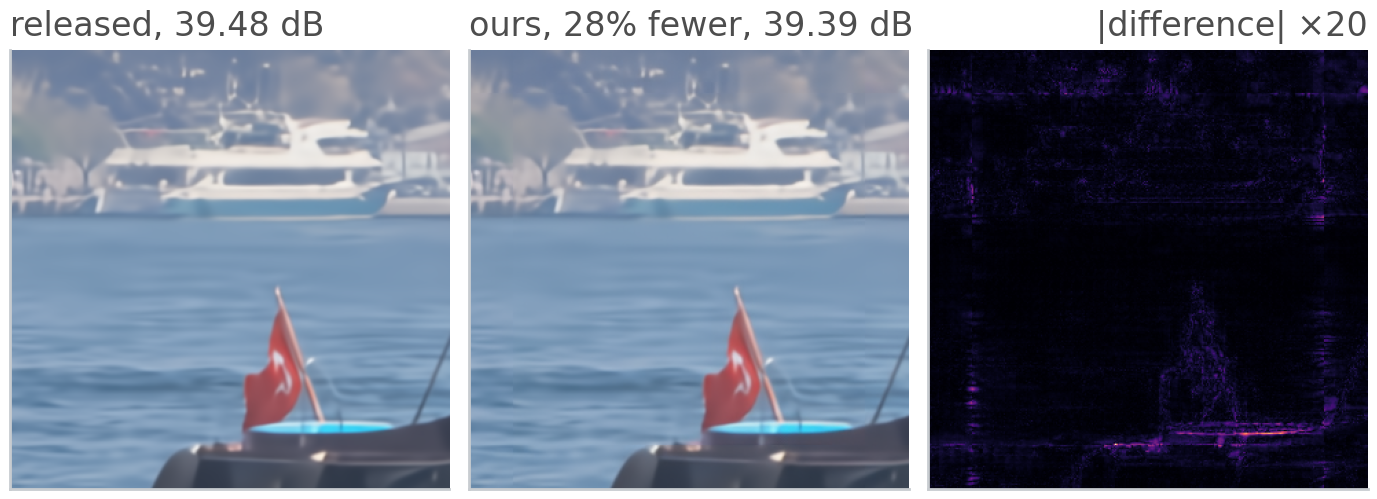
\includegraphics[width=\columnwidth]{figures/qualitative.png}
\caption{\textbf{What the saving looks like.} The same bitstream decoded by the released decoder and by ours at the 0.1 dB operating point. The crop is the tile that gave up the most quality on this frame, chosen automatically rather than by eye, so it shows the method's worst case here and not a flattering one.}
\end{figure}

\begin{figure}[t]
\centering
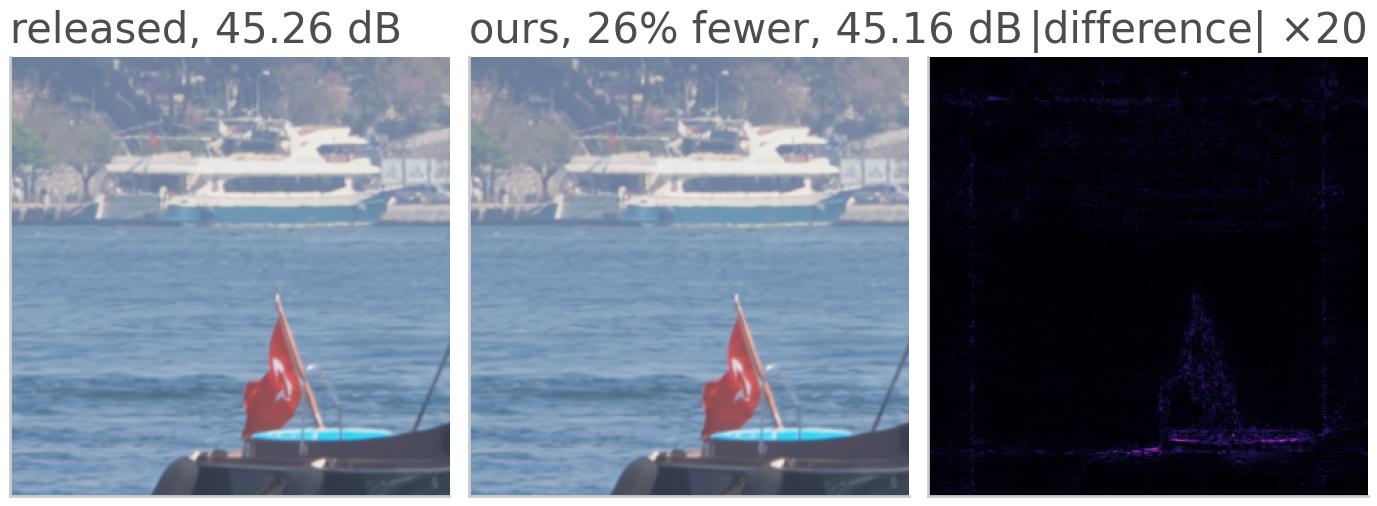
\includegraphics[width=\columnwidth]{figures/qualitative_q63.png}
\caption{\textbf{The same frame at the top of the rate range.} Bosphorus at q\QualHighQp, \QualHighBpp bpp, the same 0.1 dB budget and the same crop as the figure above. The released decoder reaches \QualHighPsnrRel dB and the routed decode \QualHighPsnrOurs dB for \QualHighDb dB delivered, and the saving is \QualHighSaving\% of the arithmetic against \QualSaving\% at q\QualQp.}
\end{figure}

The allocation is what moved between the two pictures. On this frame \QualShallowLow of 40 tiles take the shallowest exit at q\QualQp and \QualShallowHigh does at q\QualHighQp, while the deepest exit goes from \QualDeepLow tiles to \QualDeepHigh. The picture is as hard to tell apart at either rate; what changes is how much of the decoder the budget will release, which is the rate dependence of the main paper's operating-point section arriving in a single frame.

